\usetikzlibrary{patterns,patterns.meta}
\tikzset{
 invisible/.style={opacity=0},
 visible on/.code={%
  \ifthenelse{\equal{#1}{}}{%
   \tikzset{alt={<\value{beamerpauses}->{}{invisible}}}%
  }{%
   \tikzset{alt={#1{}{invisible}}}%
  }%
 },
 alt/.code args={<#1>#2#3}{%
  \alt<#1>{\pgfkeysalso{#2}}{\pgfkeysalso{#3}} % \pgfkeysalso doesn't change the path
 }
}

\begin{frame}
    \frametitle{\problemtitle}
    \begin{block}{Problem}
        Given a graph and the probability $p(v)$ for each store $v$ to have kruidnoten, output the expected length of a shortest path from vertex $1$ to $n$ if we get kruidnoten.
    \end{block}

    \pause

    \begin{figure}
        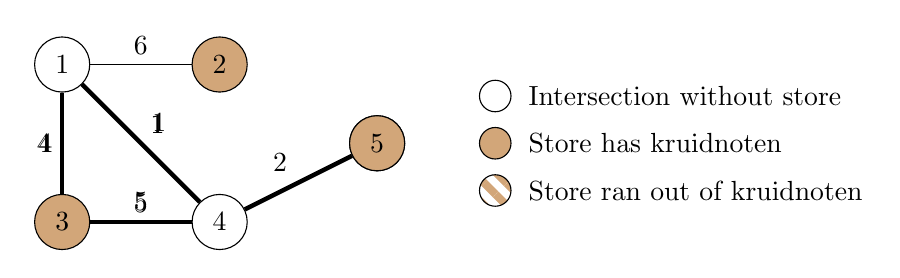
\begin{tikzpicture}[node/.style={draw, circle, minimum size=7mm}]
            \tikzstyle{hashed}=[pattern={Lines[angle=-45, distance=2mm, line width=1mm]}, pattern color=brown!70, outer sep=0pt]
            \node[node]                (1) at (0,  0) {$1$};
            \node[node, fill=brown!70] (2) at (2,  0) {$2$};
            \node[node, fill=brown!70] (3) at (0, -2) {$3$};
            \node[node]                (4) at (2, -2) {$4$};
            \node[node, hashed, visible on=<3>]        (5) at (4, -1) {$5$};
            \node[node, fill=brown!70, visible on=<2>]        (5) at (4, -1) {$5$};
            \draw              (1) -- node[above]{$6$} (2);
            \draw[ultra thick, visible on=<3>] (1) -- node[left]{$4$} (3);
            \draw[visible on=<2>] (1) -- node[left]{$4$} (3);
            \draw[visible on=<3>] (1) -- node[above right]{$1$} (4);
            \draw[ultra thick, visible on=<2>] (1) -- node[above right]{$1$} (4);
            \draw[visible on=<3>] (1) -- node[above right]{$1$} (4);
            \draw[ultra thick, visible on=<3>] (3) -- node[above]{$5$} (4);
            \draw[visible on=<2>] (3) -- node[above]{$5$} (4);

            \draw[ultra thick] (4) -- node[above left]{$2$} (5);

            \node[node, minimum size=4mm]                at (5.5, -0.4) {};
            \node[node, minimum size=4mm, fill=brown!70] at (5.5, -1.0) {};
            \node[node, minimum size=4mm, hashed]        at (5.5, -1.6) {};
            \node[anchor=west] at (5.8, -0.4) {Intersection without store};
            \node[anchor=west] at (5.8, -1.0) {Store has kruidnoten};
            \node[anchor=west] at (5.8, -1.6) {Store ran out of kruidnoten};
        \end{tikzpicture}
    \end{figure}
    \begin{block}{Idea}
        \begin{itemize}
            \item We get kruidnoten at a store if it has kruidnoten and no better store has kruidnoten.
            \item A store is better if there is a shorter path that visits the store.
        \end{itemize}
    \end{block}
\end{frame}

\begin{frame}
    \frametitle{\problemtitle}
    \begin{block}{Solution}
        \begin{itemize}
            \item<1-> For each store $v$, compute the length $d(v)$ of a shortest path if we visit the store.
            % \begin{itemize}
            %     \item Run Dijkstra from vertex $1$ and vertex $n$ to obtain the distances $\mathrm{dist}_1(v)$ and $\mathrm{dist}_n(v)$ to each store.
            %     \item Then, $d(v) = \mathrm{dist}_1(v) + \mathrm{dist}_n(v)$.
            % \end{itemize}
            \item<2-> Sort all stores by $d(v)$ in ascending order, assume $d(v_1) \leq d(v_2) \leq \ldots \leq d(v_n)$.
            \item<3-> The probability that $v_k$ has kruidnoten and no better store has them is $$p_\text{best}(v_k) = p(v_k) \cdot \prod_{i = 1}^{k - 1} (1 - p(v_i))~.$$
            \item<4-> The expected length of a shortest path if we get kruidnoten is $$\sum_{k=1}^{n} p_\text{best}(v_k) \cdot d(v_k)~.$$
        \end{itemize}
        \visible<5->{Running time: $\mathcal O(m \log(n))$}
    \end{block}
    \visible<6->{\solvestats}
\end{frame}
